\section{Complex Functions as Mappings}
\label{sec:ch5-complex-functions}

A complex function maps one plane to another:
\[
w=f(z),\qquad z=x+iy,\qquad w=u+iv.
\]
Equivalently, $u=u(x,y)$ and $v=v(x,y)$. The function therefore transforms points, curves, angles, and regions.

For $f(z)=z^2$,
\[
(x+iy)^2=(x^2-y^2)+i(2xy),
\]
so
\[
u=x^2-y^2,\qquad v=2xy.
\]
In polar form, $z=re^{i\theta}$ gives $w=r^2e^{i2\theta}$: radii are squared and angles are doubled.

\begin{figure}[htbp]
\centering
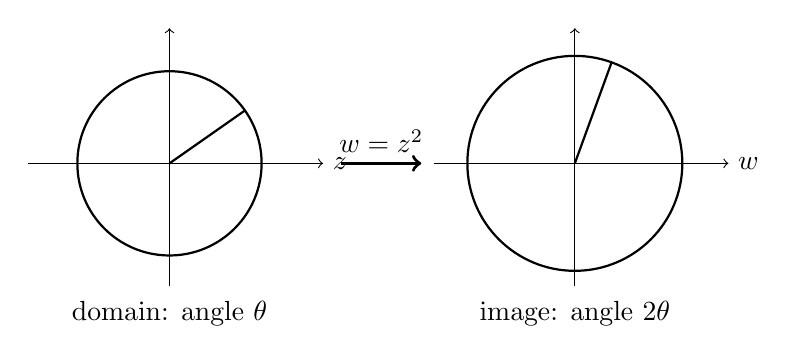
\begin{tikzpicture}[scale=0.78]
\begin{scope}
\draw[->] (-2.3,0)--(2.5,0) node[right] {$z$}; \draw[->] (0,-2.0)--(0,2.2);
\draw[thick] (0,0) circle (1.5); \draw[thick] (0,0)--({1.5*cos(35)},{1.5*sin(35)});
\node at (0,-2.45) {domain: angle $\theta$};
\end{scope}
\draw[->,very thick] (2.8,0)--(4.1,0) node[midway,above] {$w=z^2$};
\begin{scope}[xshift=6.6cm]
\draw[->] (-2.3,0)--(2.5,0) node[right] {$w$}; \draw[->] (0,-2.0)--(0,2.2);
\draw[thick] (0,0) circle (1.75); \draw[thick] (0,0)--({1.75*cos(70)},{1.75*sin(70)});
\node at (0,-2.45) {image: angle $2\theta$};
\end{scope}
\end{tikzpicture}

\caption{The map $w=z^2$ doubles arguments and squares moduli.}
\label{fig:ch5-square-map}
\end{figure}

Basic geometric maps include
\begin{align}
f(z)&=z+a &&\text{translation},\\
f(z)&=az &&\text{rotation and scaling},\\
f(z)&=\bar z &&\text{reflection},\\
f(z)&=\frac{1}{z} &&\text{inversion with angular reversal}.
\end{align}
The linear fractional or M\"obius transformation
\[
f(z)=\frac{az+b}{cz+d},\qquad ad-bc\neq0,
\]
combines translations, rotations, dilations, and inversion. Such maps send generalized circles---circles or straight lines---to generalized circles.

\begin{figure}[htbp]
\centering
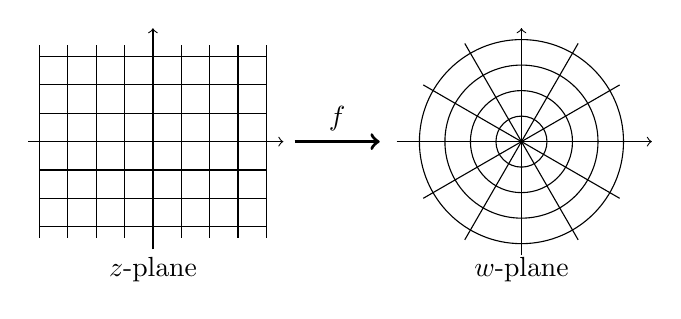
\begin{tikzpicture}[scale=0.72]
\begin{scope}
\draw[step=.5,thin] (-2,-1.7) grid (2,1.7); \draw[->] (-2.2,0)--(2.3,0); \draw[->] (0,-1.9)--(0,2);
\node at (0,-2.25) {$z$-plane};
\end{scope}
\draw[->,very thick] (2.5,0)--(4.0,0) node[midway,above] {$f$};
\begin{scope}[xshift=6.5cm]
\draw[->] (-2.2,0)--(2.3,0); \draw[->] (0,-1.9)--(0,2);
\foreach \r in {.45,.9,1.35,1.8}{\draw[thin] (0,0) circle (\r);}
\foreach \a in {0,30,...,150}{\draw[thin] ({-2*cos(\a)},{-2*sin(\a)})--({2*cos(\a)},{2*sin(\a)});}
\node at (0,-2.25) {$w$-plane};
\end{scope}
\end{tikzpicture}

\caption{A preview of a M\"obius transformation: grid geometry is reorganized while local angle structure is preserved away from singular points.}
\label{fig:ch5-mobius-preview}
\end{figure}

\begin{keyidea}[A function is more than a formula]
On the real line, a graph often captures a function. For $f:\mathbb C\to\mathbb C$, a graph would require four real dimensions. The useful replacement is to study how the function maps families of curves, domains, and local grids.
\end{keyidea}
